\documentclass[12pt, titlepage]{article}

\usepackage{amsmath, mathtools}
\usepackage[round]{natbib}
\usepackage{amsfonts}      
\usepackage{amssymb}
\usepackage{graphicx}
\usepackage{colortbl}
\usepackage{xr}
\usepackage{hyperref}
\usepackage{longtable}
\usepackage{xfrac}
\usepackage{tabularx}
\usepackage{float}
\usepackage{siunitx}
\usepackage{booktabs}
\usepackage{multirow}
\usepackage{caption}
\usepackage{fullpage}

\hypersetup{
bookmarks=true,     % show bookmarks bar?
colorlinks=true,       % false: boxed links; true: colored links
linkcolor=red,          % color of internal links (change box color with linkbordercolor)
citecolor=blue,        % color of links to bibliography
filecolor=magenta,  % color of file links
urlcolor=cyan          % color of external links
}

\usepackage{array}

%% Comments

\usepackage{color}

\newif\ifcomments\commentstrue

\ifcomments
\newcommand{\authornote}[3]{\textcolor{#1}{[#3 ---#2]}}
\newcommand{\todo}[1]{\textcolor{red}{[TODO: #1]}}
\else
\newcommand{\authornote}[3]{}
\newcommand{\todo}[1]{}
\fi

\newcommand{\wss}[1]{\authornote{blue}{SS}{#1}}
\newcommand{\an}[1]{\authornote{magenta}{Malavika}{#1}}


\newcounter{stepnum} %Likely change number
\newcommand{\lthestepnum}{step\thestepnum}
\newcommand{\stepref}[1]{step\ref{#1}}

\newcommand{\progname}{SFS}

\begin{document}

\title{Module Interface Specification for Software for Fraction Solid}

\author{Spencer Smith, Malavika Srinivasan and Vincent Cherk}

\date{\today}

\maketitle

\pagenumbering{roman}

\section{Symbols, Abbreviations and Acronyms}

See SRS Documentation at
\url{https://gitlab.cas.mcmaster.ca/SEforSC/se4sc/tree/git-svn/GradStudents/Malavika/SRSSFS}

\newpage

\tableofcontents

\newpage

\pagenumbering{arabic}

\section{Introduction}

The following document details the Module Interface Specifications for the
implemented modules in a program simulating the fraction of solid formed during
the casting process over time. It is intended to ease navigation through the
program for design and maintenance purposes.

Complementary documents include the System Requirement Specifications and Module
Guide.  The full documentation and implementation can be found at
\url{https://gitlab.cas.mcmaster.ca/SEforSC/se4sc/tree/git-svn/GradStudents/Malavika}.

The specification is given in terms of functions, rather than sequences.  For
instance, the predicted fraction of the solid is given as a function of time
($\mathbb{R} \rightarrow \mathbb{R})$, not as a sequence ($\mathbb{R}^n$).  This
approach is more straightforward for the specification, but in the
implementation stage, it will likely be necessary to introduce to introduce a
sequence, assuming that a numerical solver is used for the system of ODEs.

\section{Notation}

The structure of the MIS for modules comes from \citet{HoffmanAndStrooper1995},
with the addition that template modules have been adapted from
\cite{GhezziEtAl2003}.  The mathematical notation comes from Chapter 3 of
\citet{HoffmanAndStrooper1995}.  For instance, the symbol := is used for a
multiple assignment statement and conditional rules follow the form
$(c_1 \Rightarrow r_1 | c_2 \Rightarrow r_2 | ... | c_n \Rightarrow r_n )$.

The following table summarizes the primitive data types used by \progname. 

\begin{center}
\renewcommand{\arraystretch}{1.2}
\noindent 
\begin{tabular}{l l p{7.5cm}} 
  \toprule 
  \textbf{Data Type} & \textbf{Notation} & \textbf{Description}\\ 
  \midrule
  character & char & a single symbol or digit\\
  integer & $\mathbb{Z}$ & a number without a fractional component in (-$\infty$, $\infty$) \\
  natural number & $\mathbb{N}$ & a number without a fractional component in [0, $\infty$) \\
  real & $\mathbb{R}$ & any number in (-$\infty$, $\infty$)\\
  \bottomrule
\end{tabular} 
\end{center}

\noindent
The specification of \progname \ uses some derived data types: sequences,
strings, and tuples. Sequences are lists filled with elements of the same data
type. Strings are sequences of characters. Tuples contain a list of values,
potentially of different types.  \progname \ also uses some user defined data
types, as given in the MIS that follows.

\section{Module Decomposition}

The following table is taken directly from the Module Guide document for this
project.  \wss{This table has to be updated when the MG is complete.}

\begin{table}[h!]
\centering
\begin{tabular}{p{0.3\textwidth} p{0.6\textwidth}}
\toprule
\textbf{Level 1} & \textbf{Level 2}\\
\midrule

{Hardware-Hiding} & ~ \\
\midrule

\multirow{7}{0.3\textwidth}{Behaviour-Hiding} 
& Control Module\\
& Configuration Module\\
& Experiment Module\\
& Parameter Specification Module\\
& Temperature Module\\
& Phase Change Points Module\\
& Calculation Module\\
& Load Module\\
& Output Verification Module\\
& Output Module\\

\midrule

\multirow{3}{0.3\textwidth}{Software Decision}
& Piecewise Data Structure Module\\
& Sequence Services Module\\
& Interpolation Module\\
& Linear Regression Module\\
& ODE Solver Module\\
& Plot Module\\

\bottomrule

\end{tabular}
\caption{Module Hierarchy}
\label{TblMH}
\end{table}

\newpage

\bibliographystyle {plainnat}
\bibliography {MIS}

\newpage

\section{MIS of Control Module} \label{Main}

\subsection{Module}

main \wss{Control is actually handled by the GUI.  See documentation by capstone
  team}

\subsection{Uses}

config(\ref{config}), expt(\ref{expt}), specParam(\ref{specParam}),
temp(\ref{temp}), calc(\ref{calc}), verifyOutput(\ref{VerifyOutput}),
Output(\ref{Output}), interp(\ref{interp}),
LinerReg(\ref{LinerReg}), ODE(\ref{ODE}).

\subsection{Syntax}

\subsubsection{Exported Access Programs}

\begin{center}
\begin{tabular}{p{2cm} p{4cm} p{4cm} p{2cm}}
\hline
\textbf{Name} & \textbf{In} & \textbf{Out} & \textbf{Exceptions} \\
\hline
main & - & - & - \\
\hline
\end{tabular}
\end{center}

\subsection{Semantics}

\subsubsection{Environment Variables}

mode: $\mathbb{R}$

inputFile: sequence of string \\ 


\subsubsection{State Variables}

None

\subsubsection{Access Routine Semantics}

\noindent main():

\begin{itemize}
\item transition: 
\end{itemize}

\textbf{Mode = Config:}
  
\begin{itemize}  
  
\item[Step \refstepcounter{stepnum}\thestepnum \label{step_params}:] Obtain the
  Parameter specification values by using parameter specification
  module (\ref{specParam}):\\

\noindent Get (filenameParam: string) \\

\item[Step \refstepcounter{stepnum}\thestepnum \label{step_config}:]Modify the
  state of the variables for the config(Section~\ref{config}) module by:\\

\noindent Get (filenameIn: string) \\

\item[Step \refstepcounter{stepnum}\thestepnum \label{step_configverify}:]Verify
  the state variables of the config module against their range obtained in step
  \ref {step_params}:\\

\end{itemize}
  
\textbf{Mode = Calib:}\\

\begin{itemize}

\item[Step \refstepcounter{stepnum}\thestepnum \label{step_matpropInput}:] Get
  the material properties for the known alloy and modify the state of the
  variables for the experiment module (\ref{expt}) by:\\

\noindent Get (filenameExp: string) \ms{This is for the material properties of the known alloy.} \\

\item[Step \refstepcounter{stepnum}\thestepnum \label{step_TempInCalib}:] Modify
  the state variables (coefficients, $T_L$, $T_S$) for the Temperature module by
  obtaining temperature data of the calibration experiment and verify them as an
  when read.\\

\noindent Get (filenamecalib: string)\\

\item[Step \refstepcounter{stepnum}\thestepnum \label{step_findh(t)}:] Modify
  the state variables of the experiment module (\ref{expt}) by finding $h$ using
  calculate\_h()  from calculate module (\ref{calc}) and Temperature
  module (\ref{temp}).
  
\end{itemize}  
  
\noindent
\textbf{Mode = Calc:}\\    

\begin{itemize}

\item[Step \refstepcounter{stepnum}\thestepnum \label{step_TempInCalc}:] Modify
  the state variables (coefficients, $T_L$, $T_S$) for the Temperature module by
  obtaining temperature data of the calculation experiment and verify them as an
  when read.\\

\noindent Get (filenamecalc: string)\\

\item[Step \refstepcounter{stepnum}\thestepnum \label{step_alpha}:] Modify the
  state variables of the calculate module (\ref{calc}) by finding $\alpha_b$ and
  $\alpha_e$ using the methods calculate\_$\alpha_b$() and
  calculate\_$\alpha_e$().

\item[Step \refstepcounter{stepnum}\thestepnum \label{step_InputL}:] Obtain the
  necessary inputs for calculating fraction solid - L. \ms{ Is L supposed to be
    user input?} \wss{I'm not sure what motivates this question.  R14 lists $L$
    (IM4) as an input.  Is something potentially incorrect in the SRS?}\ms{No
    Dr.Smith, SRS says "input L" but does not say whether it is from user or to
    be calculated.I guess it should be user input. I get this question because
    in SRS, L is listed along with $\alpha$, $\rho$ and $C_v$ , some of which
    are supposed to be calculated.}

\item[Step \refstepcounter{stepnum}\thestepnum \label{step_fs}:]Calculate fs
  using the method calculate\_FS()   in calculate module (\ref{calc}), ODE Solver
  module (\ref{ODE}) and Temperature module (\ref{temp}).

\item[Step \refstepcounter{stepnum}\thestepnum \label{step_verifyOutput}:]
  Verify the fraction solid output using the output verification
  module (\ref{VerifyOutput}).

\item[Step \refstepcounter{stepnum}\thestepnum \label{step_output}:] Output the
  fraction solid results of calibration and calculation to respective output
  files using the output module (\ref{Output}).

\item[Step \refstepcounter{stepnum}\thestepnum \label{step_plot}:] Plot the
  fraction solid with respect to time, temperature and cooling rate.  Plotting
  will be handled by  as per
  requirement using plotting module (\ref{Plot}). 

\end{itemize}

\newpage

\section{MIS of Configuration Module} \label{config}

The secrets of this module are the data structure for input parameters for the c , how the
values are input and how the values are verified.  The load and verify secrets
are isolated to their own access programs.

\subsection{Module}

config

\subsection{Uses}

SpecParam (Section~\ref{specParam})

\subsection{Syntax}

\begin{tabular}{p{3cm} p{1cm} p{1cm} >{\raggedright\arraybackslash}p{9cm}}
\toprule
\textbf{Name} & \textbf{In} & \textbf{Out} & \textbf{Exceptions} \\
\midrule
load\_params & string & - &  FileError\\
verify\_params & - & - & ValueError\\
$H$ & - & $\mathbb{R}$\\
$D$ & - & $\mathbb{R}$\\
$n$ & - & $\mathbb{N}$\\
$y_{TC}$ & - & $\mathbb{R}^n$\\
$dt$ & - & $\mathbb{R}$ \\
$dy$ & - & $\mathbb{R}$\\

\bottomrule
\end{tabular}

\subsection{Semantics}

\subsubsection{Environment Variables}

inputFile: sequence of string

\subsubsection{State Variables}

\renewcommand{\arraystretch}{1.2}
\begin{longtable*}[l]{l} 
\# From R1\\
$H$: $\mathbb{R}$ \\
$D$: $\mathbb{R}$ \\
$n$: $\mathbb{R}$ \\
$y_{TC}$: $\mathbb{R}^n$ \\
$dt$: $\mathbb{R}$ \\
$dy$: $\mathbb{R}$\\
\end{longtable*}

\subsubsection{Assumptions}

\begin{itemize}

\item load\_params will be called before the values of any state variables will be accessed.

\end{itemize}

\subsubsection{Access Routine Semantics}

\noindent config.$H$:
\begin{itemize}
\item output: \textit{out} := $H$
\item exception: None
\end{itemize}

\noindent config.$D$:
\begin{itemize}
\item output: \textit{out} := $D$
\item exception: None
\end{itemize}

\noindent config.$n$:
\begin{itemize}
\item output: \textit{out} := $n$
\item exception: None
\end{itemize}

\noindent config.$dt$:
\begin{itemize}
\item output: \textit{out} := $dt$
\item exception: None
\end{itemize}


\noindent config.$dy$:
\begin{itemize}
\item output: \textit{out} := $dy$
\item exception: None
\end{itemize}

\noindent config.$y_{TC}$:
\begin{itemize}
\item output: \textit{out} := $y_{TC}$
\item exception: None
\end{itemize}

\noindent load\_params($s$):
\begin{itemize}
\item transition: {inputFile} is used to modify the state variables using the
  following procedural specification:

\begin{enumerate}

\item Read data sequentially from inputFile to populate the state variables from
  R1 ($H$ to $y_{TC}$).

\item verify\_params()

\end{enumerate}

\item exception: exc := a file name $s$ cannot be found OR the format of
  inputFile is incorrect $\Rightarrow$ FileError

\end{itemize}

\noindent verify\_params():
\begin{itemize}
\item exception: exc := 
\end{itemize}

\begin{tabular}{p{13cm} p{2.75cm}}

\toprule
\textbf{Name}&\textbf{Exception}\\
\midrule

$\neg (H_{\text{min}} \leq H \leq H_{\text{max}})$ & $\Rightarrow$ ValueError\\
$\neg (D_{\text{min}} \leq D \leq D_{\text{max}})$ & $\Rightarrow$ ValueError\\
$n > n_{max}$ & $\Rightarrow$ ValueError\\
$\neg (dt_{\text{min}} \leq dt \leq dt_{\text{max}})$ & $\Rightarrow$ ValueError\\
$\neg (\forall (i: \mathbb{N} | i \in [1..n-1] \cdot 0 \leq {y_{TC}}_i < H
  \wedge {y_{TC}}_i < {y_{TC}}_{i+1}) \wedge {y_{TC}}_n \leq H)$ & $\Rightarrow$ ValueError\\

\bottomrule
\end{tabular}\\
~\\

\noindent This table is based on the information in Table 1 (Input Variables for
Configuration Mode) from the SRS.

\subsection{Considerations}

The value of each state variable can be accessed through its name (getter).  An
access program is available for each state variable.  There are no setters for
the state variables, since the values will be set and checked by the
load\_params access program, and the values will not changed for the life of the
program.

For each of the possible ValueError exceptions, a string describing the invalid input
should be attached the exception.

\newpage

\section{MIS of Experiment Module } \label{expt}

\subsection{Template Module}

expt

\subsection{Uses}

SpecParam (Section~\ref{specParam})

\subsection{Syntax}

\begin{tabular}{p{3cm} p{3cm} p{1cm} >{\raggedright\arraybackslash}p{9cm}}
\toprule
\textbf{Name} & \textbf{In} & \textbf{Out} & \textbf{Exceptions} \\
\midrule
load\_params\_calib & string & - &  FileError \\
load\_params\_calc & string & - &  FileError \\
\midrule
\textbf{Getters} & & &\\
\midrule
$k_{S}$ & - & $\mathbb{R}$& \\
$k_{L}$ & - & $\mathbb{R}$ & \\
$C_{p}^L$ & - & $\mathbb{R}$& \\
$C_p^S$ & - & $\mathbb{R}$& \\
$\rho_S$ & - & $\mathbb{R}$& \\
$\rho_L$ & - & $\mathbb{R}$& \\
$\alpha_S$ & - & $\mathbb{R}$& \\
$\alpha_L$ & - & $\mathbb{R}$& \\
$T_{\text{env}}$ & - & $\mathbb{R}$& \\
$h$&-&$\mathbb{R}$& \\
\midrule
\textbf{Setters} & & &\\
\midrule
$k_{S}$ & $\mathbb{R}$ & & ValueError\\
$k_{L}$ & $\mathbb{R}$ & & ValueError\\
$C_{p}^L$ & $\mathbb{R}$ & & ValueError\\
$C_p^S$ & $\mathbb{R}$ & & ValueError\\
$\rho_S$ & $\mathbb{R}$ & & ValueError\\
$\rho_L$ & $\mathbb{R}$ & & ValueError\\
$\alpha_S$ & $\mathbb{R}$ & & ValueError\\
$\alpha_L$ & $\mathbb{R}$ & & ValueError\\
$T_{\text{env}}$ & $\mathbb{R}$ & & ValueError\\
$h$ & $\mathbb{R}$ & & ValueError\\
\bottomrule
\end{tabular}

\subsection{Semantics}

\subsubsection{State Variables}

$k_{S}$ : $\mathbb{R}$\\
$k_{L}$ :  $\mathbb{R}$\\
$C_{p}^L$ :  $\mathbb{R}$\\
$C_p^S$ :  $\mathbb{R}$\\
$\rho_S$ :  $\mathbb{R}$ \\
$\rho_L$ :  $\mathbb{R}$\\
$\alpha_S$ :  $\mathbb{R}$\\
$\alpha_L$ :  $\mathbb{R}$\\
$T_{\text{env}}$ :  $\mathbb{R}$\\
$h$: $\mathbb{R}$\\

\subsubsection{Assumptions}

A setter will be called for a given state variable before the corresponding
getter is called.

\subsubsection{Access Routine Semantics}

\noindent load\_params\_calib($s$):
\begin{itemize}
\item transition:  {inputFile1} is used to modify the state variables using the following procedural specification:

\begin{enumerate}

\item Read data sequentially from inputFile to populate the state variables from
  R7 ($k_S$ to $T_{\text{env}}$).
\item Use setters defined in this module, so that appropriate exceptions will be generated

\end{enumerate}

\item exception: exc := a file name $s$ cannot be found OR the format of
  inputFile is incorrect $\Rightarrow$  FileError

\end{itemize}

\noindent load\_params\_calc($s$):
\begin{itemize}
\item transition:  {inputFile2} is used to modify the state variables using the following procedural specification:

\begin{enumerate}

\item Read data sequentially from inputFile to populate the state variables from
  R7 ($k_S$ to $h$).
\item Use setters defined in this module, so that appropriate exceptions will be
  generated

\end{enumerate}

\item exception: exc := a file name $s$ cannot be found OR the format of
  inputFile is incorrect $\Rightarrow$  FileError

\end{itemize}

\textbf{Getters}\\

\noindent expt.$k_{S}$:
\begin{itemize}
\item output: \textit{out} := $k_{S}$
\item exception: none
\end{itemize}

\noindent expt.$k_{L}$:
\begin{itemize}
\item output: \textit{out} := $k_{L}$
\item exception: none
\end{itemize}

\noindent expt.$C_{p}^L$:
\begin{itemize}
\item output: \textit{out} := $C_{p}^L$
\item exception: none
\end{itemize}

\noindent expt.$C_p^S$:
\begin{itemize}
\item output: \textit{out} := $C_p^S$
\item exception: none
\end{itemize}

\noindent expt.$\rho_S$:
\begin{itemize}
\item output: \textit{out} := $\rho_S$
\item exception: none
\end{itemize}

\noindent expt.$\rho_L$:
\begin{itemize}
\item output: \textit{out} := $\rho_L$
\item exception: none
\end{itemize}

\noindent expt.$\alpha_S$:
\begin{itemize}
\item output: \textit{out} := $\alpha_S$
\item exception: none
\end{itemize}

\noindent expt.$\alpha_L$:
\begin{itemize}
\item output: \textit{out} := $\alpha_L$
\item exception: none
\end{itemize}

\noindent expt.$T_{\text{env}}$:
\begin{itemize}
\item output: \textit{out} := $T_{\text{env}}$
\item exception: none
\end{itemize}

\noindent expt.$h$:
\begin{itemize}
\item output: \textit{out} := $h$
\item exception: none
\end{itemize}
~\\

\noindent \textbf{Setters}\\

There is also a corresponding setter for each state variable.  When setting the
values the validity will be checked, following Table 3 (Input Variables for
Material Properties and Operating Conditions) in the SRS.  Any invalid inputs
will generate a Value Error with a corresponding string message describing the
reason the data is considered invalid.

\subsection{Considerations}

The state variables for the material properties and processing conditions are
currently constants.  In the future some of the variables may be changed to have
function types ($\mathbb{R} \rightarrow \mathbb{R}$).

\newpage

\section{MIS of Parameter Specification Module} \label{specParam}

\subsection{Module}

specParam

\subsection{Uses}

None

\subsection{Syntax}

\subsubsection{Exported constants}

\#From the Table 6 in SRS\\
\noindent
  $\mbox{AbsZero}$ :=  273.15\\
  $H_{\mbox{min}}$ := 0.001\\
  $H_{\mbox{max}}$ := 100 \\
  $D_{\mbox{min}}$ := 0.001 \\
  $D_{\mbox{max}}$ := 100 \\
  $m_{\mbox{max}}$ := 1000\\
  $dt_{\mbox{min}}$ := 0.0001\\
  $dt_{\mbox{max}}$:=  1000 \\
  $n_{\mbox{max}}$:= $1 \times 10^4$\\
  $T_{\mbox{min}}$:=   100 \\
  $T_{\mbox{max}}$:=   $1 \times 10^4$ \\
  ${k_S}_{\mbox{min}}$:=  0.001 \\
  ${k_S}_{\mbox{max}}$:=  $1 \times 10^5$\\
  ${k_L}_{\mbox{min}}$:=  0.001 \\
  ${k_L}_{\mbox{max}}$:=  $1 \times 10^5$\\
  ${\rho_S}_{\mbox{min}}$:=  0.001 \\
  ${\rho_S}_{\mbox{max}}$:=  $1 \times 10^4$\\
  ${\rho_L}_{\mbox{min}}$ := 0.001\\
  ${\rho_L}_{\mbox{max}}$ := $1 \times 10^4$\\
  ${C_P^S}_{\mbox{min}}$ := $1 \times 10^{-4}$\\
  ${C_P^S}_{\mbox{max}}$ := $1 \times 10^{4}$\\
   ${C_P^L}_{\mbox{min}}$ := $1 \times 10^{-4}$\\
  ${C_P^L}_{\mbox{max}}$ := $1 \times 10^{4}$ \\
  ${C_v^L}_{\mbox{min}}$:=  $1 \times 10^{-4}$ \\
  ${C_v^L}_{\mbox{max}}$ := $1 \times 10^{4}$\\
  ${C_v^S}_{\mbox{min}}$:=  $1 \times 10^{-4}$ \\
  ${C_v^S}_{\mbox{max}}$ := $1 \times 10^{4}$ \\
  $L_{\mbox{min}}$:=  0.001 \\
  $L_{\mbox{max}}$ := $1 \times 10^{10}$ \\
  ${T_{\mbox{env}}}_{\mbox{min}}$ := 0 \\
  ${T_{\mbox{env}}}_{\mbox{max}}$ := 100\\
  
\subsubsection{Assumptions}

None

\subsubsection{Access Routine Semantics}

N/A

\newpage

\section{MIS of Temperature Module} \label{temp}

\subsection{Module}

TData

\subsection{Uses}

config, PiecewiseADT for PiecewiseT, Load, SeqServices

\subsubsection* {Exported Constants}

$\Delta t = 1 \times 10^{-5}$\\ %These might make sense as state variables?
$\Delta y = 1 \times 10^{-3}$

\subsection{Syntax}

\subsubsection{Exported Access Programs}

\begin{center}
\begin{tabular}{p{3cm} p{5cm} p{5cm} p{3.5cm}}
\toprule
\textbf{Name} & \textbf{In} & \textbf{Out} & \textbf{Exceptions} \\
\midrule
TData\_init & & ~ & ~ \\
%\hline
TData\_add & $s: \mbox{PiecewiseT}$, $y: \mathbb{R}$, $t^*_L: \mathbb{R}$, $T^*_L:
             \mathbb{R}$, $t^*_S: \mathbb{R}$, $T^*_S: \mathbb{R}$ & ~ & IndepNotAscending\\
%\hline
TData\_rm & $i: \mathbb{N}$ &  & InvalidIndex\\
%\hline
TData\_getC & $i: \mathbb{N}$ & PiecewiseT & InvalidIndex\\
%\hline
TData\_getLiq & $i: \mathbb{N}$ & $\mathbb{R}$, $\mathbb{R}$ & InvalidIndex\\
%\hline
TData\_getSol & $i: \mathbb{N}$ & $\mathbb{R}$, $\mathbb{R}$ & InvalidIndex\\
%\hline
TData\_slice & $t: \mathbb{R}$ & seq of $\mathbb{R}$, seq of $\mathbb{R}$ & ~\\
%\hline
TData\_breakPts &  & seq of $\mathbb{R}$, seq of $\mathbb{R}$, seq of $\mathbb{R}$ & ~\\
%\hline
TData\_T &  $y: \mathbb{R}$, $t: \mathbb{R}$ & $\mathbb{R}$ & OutOfDomain\\
%\hline
TData\_dTdt &  $y: \mathbb{R}$, $t: \mathbb{R}$ & $\mathbb{R}$ & OutOfDomain\\
%\hline
TData\_d2Tdy2  &   $y: \mathbb{R}$, $t: \mathbb{R}$ & $\mathbb{R}$ & OutOfDomain\\
\bottomrule
\end{tabular}
\end{center}

\subsection{Semantics}

\subsubsection{State Variables}

$S$: sequence of PiecewiseT\\ 
$Y$: sequence of $\mathbb{R}$\\
$t_L$: sequence of $\mathbb{R}$\\
$T_L$: sequence of $\mathbb{R}$\\
$t_S$: sequence of $\mathbb{R}$\\
$T_S$: sequence of $\mathbb{R}$

\subsubsection{State Invariants}

None

\subsubsection{Assumptions}

TData\_init() will be called before any other access programs.

\subsubsection{Access Routine Semantics}

TData\_init():
\begin{itemize}
\item transition: $S, Y, t_L, T_L, t_S, T_S  := < >, <>, <>, <>$
\item exception: none
\end{itemize}

\noindent TData\_add($s, y, t^*_L, T^*_L, t^*_S, T^*_S$):
\begin{itemize}
\item transition: $S, Y, t_L, T_L, t_S, T_S  := S || <s>, Y || <y>, t_L ||
  <t^*_L>, T_L|| <T^*_L>, t_S|| <t^*_S>, T_S|| <T^*_S>$
\item exception: $exc := ( |Y| > 0 \wedge y \leq Y_{|Y|-1} \Rightarrow
  \mbox{IndepNotAscending})$
\end{itemize}

\noindent TData\_rm($i$):
\begin{itemize}
\item transition: $s := s[0..i-1] || s[i+1..|s|-1]$
\item exception:  $exc := (\neg(0 \leq i < |S|-1) \Rightarrow \mbox{InvalidIndex})$
\end{itemize}

\noindent TData\_getC($i$):
\begin{itemize}
\item output: $out := S[i]$
\item exception: $exc := (\neg(0 \leq i < |S|-1) \Rightarrow \mbox{InvalidIndex})$
\end{itemize}

\noindent TData\_Liq($i$):
\begin{itemize}
\item output: $out := t_L[i], T_L[i]$
\item exception: $exc := (\neg(0 \leq i < |S|-1) \Rightarrow \mbox{InvalidIndex})$
\end{itemize}

\noindent TData\_Sol($i$):
\begin{itemize}
\item output: $out := t_S[i], T_S[i]$
\item exception: $exc := (\neg(0 \leq i < |S|-1) \Rightarrow \mbox{InvalidIndex})$
\end{itemize}

\noindent TData\_slice($t$):
\begin{itemize}
\item output: $out := \langle Y_0, Y_1, ..., Y_{|Y|-1} \rangle, \langle
  S_0.\mbox{feval}(t), S_1.\mbox{feval}(t), ..., S_{|S|-1}.\mbox{feval}(t)
  \rangle$
\item exception: None
\end{itemize}

\noindent TData\_breakPts():
\begin{itemize}
\item output: $out := \langle Y_0, Y_1, ..., Y_{|Y|-1} \rangle, \langle
  S_0.x_1, S_1.x_1, ..., S_{|S|-1}.x_1 \rangle, \langle S_0.x_2, S_1.x_2, ..., S_{|S|-1}.x_2
  \rangle$
\item exception: None
\end{itemize}

\noindent TData\_T($t, y$):
\begin{itemize}
\item output: Find $out$ using the following steps:
\begin{enumerate}
\item Using TData\_breakPts() and interpolation determine the approximate values
  for the breakpoints ($t_1^\text{approx}$, $t_1^\text{approx}$) for the curve
  at height $y$.
\item Determine what segment of the piecewise curve applies at time $t$.  It
  will be the first segment if $t \leq t_1^\text{approx}$, the second segment if
  $t_1^\text{approx} < t \leq t_2^\text{approx}$ and the third segment if
  $t_2^\text{approx} < t$.
\item Use the curves in $S$ that are in the same segment (first, second or
  third) at given by the $t$ and $y$ combination.  Use the data from these
  curves to interpolate the required $out$ value.
\end{enumerate}
\item exception: $exc := (\neg \mbox{isInBounds}(Y, y) \Rightarrow \mbox{OutOfDomain})$
\end{itemize}

\noindent dTdt($t, y$):
\begin{itemize}
\item output: \textit{out} := $\frac{T(y, t + \Delta t) - T(y, t)}{\Delta t}$
\item exception: $exc := (\neg \mbox{isInBounds}(Y, y) \Rightarrow \mbox{OutOfDomain})$
\end{itemize}

\noindent d2Tdy2($t, y$):
\begin{itemize}
\item output: \textit{out} := $\frac{T(y - \Delta y, t) + T(y + \Delta y, t) - 2 * T(y,
    t)}{\Delta y^2}$
\item exception: $exc := (\neg \mbox{isInBounds}(Y, y) \Rightarrow \mbox{OutOfDomain})$
\end{itemize}

\newpage

\section{MIS of Identify Points Module} \label{bkpt}

\subsection{Module}

IdentifyPts

\subsection{Uses}

None

\subsection{Syntax}

\subsubsection{Exported Access Programs}

\begin{center}
\begin{tabular}{p{3cm} p{2cm} p{4cm} p{2cm}}
\hline
\textbf{Name} & \textbf{In} & \textbf{Out} & \textbf{Exceptions} \\
\hline
find\_breakPts & $x$: seq of $\mathbb{R}$, $y$: seq of $\mathbb{R}$ & $\mathbb{R}$, $\mathbb{R}$ & \\
find\_liquidus & $s: \mbox{string}$ & seq of $\mathbb{R}$, seq of $\mathbb{R}$ & \\
find\_solidus & $s: \mbox{string}$ & seq of $\mathbb{R}$, seq of $\mathbb{R}$ & \\
\hline
\end{tabular}
\end{center}

\subsection{Semantics}

\subsubsection{State Variables}

None

\subsubsection{Assumptions}

\subsubsection{Access Routine Semantics}

\noindent find\_breakPts($T$)

\begin{itemize}
\item output: Given the sequence $T$ identify the two points where there is a
  discontinuity in the slope.  Return these two points, which can then be used
  as the initial guesses for $x_1$ and $x_2$.  Hopefully the points can be
  determined using the first derivative of the data and the peak detection
  utilities.  \wss{Investigation is necessary here.}
\item exception: None
\end{itemize}


\noindent find\_liquidus(s):

From the input file,         

\begin{itemize}

\item \text{for i in range 0 to 7 , calculate the following}
\begin{equation*}
\text{tempdiff}  = TC_{i+1} - TC{_i} 
\end{equation*}

\item for TC0, invert the tempdiff by ({$0 - \text{tempdiff}$}) and find the
  first peak using peakutils, the corresponding temp value at maximum
  ({$0 - \text{tempdiff}$}) is the solidus point for TC0.

\item from TC1 the solidus point is defined as the last point at which the temp
  diff is maximum. please note this does not apply to first TC.
  
\item Note down the temperature and time values.  
\item Modify the state of the variable $T_S$ and $t_S$.\\

\end{itemize}

\noindent LiquidusPoint():\\

From the input file,        

\begin{itemize}

\item calculate tempdiff as follows
\begin{equation*}
\text{tempdiff} = TC_{1} - TC_{0} 
\end{equation*}
\item find the peaks using the peakutils

\item The temperature at the first peak in tempdiff is taken as the liquidus
  temperature for all the thermocouples. 
\item Note down the temperature and time values. 
\item Modify the state of the variable $T_L$ and $t_L$.\\

\end{itemize}

\noindent liqTemp($y$):
\begin{itemize}
\item Obtain a polynomial regression between location values and the $T_L$.\\
\item Pass $y$ to this polynomial to obtain liquidus temperature ($T_L(y)$).\\
\end{itemize}

\noindent liqtime($y$):
\begin{itemize}
\item Obtain a polynomial regression between location values and the $t_L$.\\
\item Pass $y$ to this polynomial to obtain liquidus time ($t_L(y)$).\\
\end{itemize}

\noindent solTemp(y):
\begin{itemize}
\item Obtain a polynomial regression between location values and $T_S$.\\
\item Pass $y$ to this polynomial to obtain solidus temperature ($T_S(y)$).\\
\end{itemize}

\noindent soltime(y):
\begin{itemize}
\item Obtain a polynomial regression between location values and $T_S$.\\
\item Pass $y$ to this polynomial to obtain solidus time ($t_S(y)$).\\
\end{itemize}

\newpage

\section{MIS of Calculation Module} \label{calc}

\subsection{Module}

calc \wss{This module spec needs work.}

\subsection{Uses}

expt, temp

\subsection{Syntax}

\subsubsection{Exported Access Programs}

\begin{center}
\begin{tabular}{p{3cm} p{6cm} p{2cm} p{2cm}}
\hline
\textbf{Name} & \textbf{In} & \textbf{Out} & \textbf{Exceptions} \\
\hline
calculate\_h  &  temp & h(t)($\mathbb{R}^n$) & \\
calculate\_$\alpha_b$ & temp & $\alpha_b$ ($\mathbb{R}$) &\\
calculate\_$\alpha_e$ & temp & $\alpha_e$ ($\mathbb{R}$) &\\
calculate\_FS & temp, L($\mathbb{R}$), $C_v ^L (T)$($\mathbb{R}$), $C_v ^S
                (T)$($\mathbb{R}$), $\rho_L (T)$($\mathbb{R}$), $\rho_S
                (T)$($\mathbb{R}$) &  $f_s$($\mathbb{R}^n$)  & bad\_$C_v ^L$,
                                                               bad\_$C_v ^S,
                                                               bad\_f_s$\\

\hline
\end{tabular}
\end{center}

\subsection{Semantics}

\subsubsection{State Variables}

$\alpha_b$: $\mathbb{R}$ \wss{Should this module really have state variables?}\\ 
$\alpha_e$: $\mathbb{R}$\\
$f_s$: $\mathbb{R}^n$\\

\subsubsection{Assumptions}

calculate\_h, calculate\_$\alpha_b$ and calculate\_$\alpha_e$  will be called before calling calculate\_FS.

\subsubsection{Access Routine Semantics}

\noindent calc.$alpha_b$:
\begin{itemize}
\item output: \textit{out} := $alpha_b$
\item exception: none
\end{itemize}

\noindent calc.$alpha_e$:
\begin{itemize}
\item output: \textit{out} := $alpha_e$
\item exception: none
\end{itemize}

\noindent calc.$f_s$:
\begin{itemize}
\item output: \textit{out} := $f_s$
\item exception: none
\end{itemize}

\noindent calculate\_h():
\begin{itemize}
\item output: \textit{out} := h(t)
\item exception: NA
\item equation:

\text{find h(t) such that it satisfies the PDE and boundary condition below.}\\
\\
\text{PDE:}\\
\begin{equation*}
\frac{\partial T}{\partial t} = \alpha_S(T) \frac{\partial^2 T}{\partial y^2},
\mbox{ where } \alpha_S(T) = \frac{k_S(T)}{\rho_S(T) C_p^S(T)}
\end{equation*}

\text{Boundary condition:}\\
\\
\text{$q = 0$ on all boundaries, except for the
          bottom of the cylinder}\\

\begin{equation*}
q(t) = h(t)(T_0(t) - T_{\text{env}}(t))
\end{equation*}

\item Reference:\textit{from IM1 in SRS}           

\end{itemize}

\noindent calculate\_$\alpha_b$():

\begin{itemize}
\item output: \textit{out} := $\alpha_b$
\item exception: none
\item equation:
\text{find $\alpha_b$ such that the following PDE and boundary conditions are
          satisfied}
\text{PDE:}\\          
\begin{equation*}
\frac{\partial T}{\partial t} = \alpha_b \frac{\partial^2 T}{\partial y^2}
\end{equation*}

\text{Boundary condition:}\\
\\
\text{$q = 0$ on all boundaries, except for the bottom of the cylinder where,}\\

\begin{equation*}
 q(t) = h(t)(T_0(t) - T_{\text{env}}(t))
 \end{equation*}
         
\item Reference \textit{from IM2 in SRS}  

\end{itemize}

\noindent calculate\_$\alpha_e$():

\begin{itemize}

\item output: \textit{out} := $\alpha_e$
\item exception: none
\item equation:
 \text{find $\alpha_e$ such that the following PDE and boundary conditions are
          satisfied}\\
\\          
\text{PDE}\\
\\          
\begin{equation*}
\frac{\partial T}{\partial t} = \alpha_b \frac{\partial^2 T}{\partial y^2}
\end{equation*}

\text{Boundary condition:}\\
\\
\text{ $q = 0$ on all boundaries, except for the bottom of the cylinder where,}
\begin{equation*}
 q(t) = h(t)(T_0(t) - T_{\text{env}}(t))
 \end{equation*}
         
\item Reference: \textit{from IM3 in SRS}  

\end{itemize}

\noindent calculate\_FS():

\begin{itemize}

\item output: \textit{out} := $f_s$
\item exception: $bad\_f_s$
\item equation:
 \text{Solve $f_s(t)$ at location $y^*$ such that the following ODE is satisfied with $f_s(t_L)=0$:}\\
 \\
 ~\newline
\text{ODE:}\\
\\  
\begin{equation*}
\dot{f_s}(f_s, t) = \frac{C_v(f_s)}{L \rho(f_s)} \left [ \frac{\partial
            T(t)}{\partial t} - \alpha(f_s)\frac{\partial^2 T(t)}{\partial y^2}
            \right ] 
\end{equation*}            
~\newline

\text{ where}\\
$C_v(f_s) = C_v^b(1 - f_s) + C_v^e f_s$\\
 $\rho(f_s) = \rho_{b}(1 - f_s) + \rho_{e} f_s$\\
 $\alpha(f_s) = \alpha_{b}(1 - f_s) + \alpha_{e} f_s$\\
\newline 
\text{where}\\
 $C_v^b = C_v^L(T_L)$,
 $C_v^e = C_v^S(T_S)$, $\rho_b = \rho_L(T_L)$, 
 $\rho_e = \rho_S(T_S)$.
  ~\newline
  After solving the ODE, $f(t)$ and $T(t)$ are known, which means that $f(T)$ can be shown.\\
         
\item Reference: \textit{from IM4 in SRS}  

\end{itemize}






\newpage

\section{Load Module}\label{load}

\subsection {Module}

Load

\subsection {Uses}

PiecewiseADT, TData, config, IdentifyPts

\subsection {Syntax}

\subsubsection {Exported Constants}

None

\subsubsection*{Exported Access Programs}

\begin{tabular}{| l | l | l | l |}
\hline
\textbf{Routine name} & \textbf{In} & \textbf{Out} & \textbf{Exceptions}\\
\hline
parse & $s: \mbox{string}$ & ~ & ~\\
loadTData & $x: \mathbb{R}^n$, y: $\mathbb{R}^n$ & ~ & ValueError\\ 
\hline
\end{tabular}

\subsection {Semantics}

\subsubsection {Environment Variables}

infile: two dimensional sequence of text characters

\subsubsection{State Variables}

None

\subsubsection{State Invariant}

None

\subsubsection{Assumptions}

The input file will match the expected specification.

\subsubsection{Access Routine Semantics}

\noindent parse($s$)\\
\noindent loadTData($x$,$y$)
\begin{itemize}
\item transition: read data from the file infile associated with the string s.
  Use this data to update the state of the TData module.  Load will first
  initialize TData (TData.init()) before populating TData with piecewise curves,
  y value and liquidus and solidus values.  In loading the data, the following
  should be kept in mind:
\begin{itemize}
\item  The initial transient data for each thermocouple will be ignored.  The first
  data point for the thermocouples corresponds to the maximum temperature
  reading for the first (lowest value of $y$) thermocouple.
\item The time data should be the actual time, not the number of accumulated
  data points.  This will mean multiplying by the time step size from the config
  file.
\item The data should be verified against the constraints in Table 2 (Input
  Variables for Calculating $T(y, t)$ in the SRS.  That is, there should be more
  than zero data points and all temperature values should be within the
  prescribed bounds.
\item The IdentifyPts functions should be used to find the initial estimates for
  the breakpoints and the values of the liquidus and solidus times and
  temperatures.
\end{itemize}
\item exception: none
\end{itemize}

\newpage

\section{MIS of Output Verification Module} \label{VerifyOutput}

\subsection{Module}

verifyop

\subsection{Uses}

\subsection{Syntax}

\subsubsection{Exported Access Programs}

\begin{center}
\begin{tabular}{p{3cm} p{7cm} p{1cm} p{2cm}}
\hline
\textbf{Name} & \textbf{In} & \textbf{Out} & \textbf{Exceptions} \\
\hline
verify\_output & $f_s$: $\mathbb{R}_n$ &  & $bad\_f_s$\\
\hline
\end{tabular}
\end{center}

\subsection{Semantics}

\subsubsection{State Variables}

None

\subsubsection{Assumptions}

All of the fields of the input parameters structure have been assigned a
value.  

\subsubsection{Access Routine Semantics}

\noindent verify\_output($f_s$):
\begin{itemize}
\item exception: $\forall t | 0 \leq t \leq t_\text{final}$,  $f_s < 0$ or $f_s > 1$  $\rightarrow bad\_f_s$\\
\end{itemize}

\newpage

\section{MIS of Output Module} \label{Output}

\subsection{Module}

op

\subsection{Uses}

-
\subsection{Syntax}


\subsubsection{Exported Access Program}

\begin{center}
\begin{tabular}{p{3cm} p{6cm} p{2cm} p{2cm}}
\hline
\textbf{Name} & \textbf{In} & \textbf{Out} & \textbf{Exceptions} \\
\hline
output\_calib & fname: string, $t$:$\mathbb{R}^n$ ,$f_{s}(t)$:$\mathbb{R}^n$\\
output\_calc & fname: string, $t$:$\mathbb{R}^n$ ,$f_{s}(t)$:$\mathbb{R}^n$\\                 
\hline
\end{tabular}
\end{center}

\subsection{Semantics}

\subsubsection{State Variables}

$f_s: \mathbb{R}_n$ (between 0 \& 1)

\subsubsection{Environment Variables}

file1: A  file - calibration\\
file2: A  file - calculation\\

\subsubsection{Access Routine Semantics}

\noindent output\_calib(fname, $t$,$f_s$):
\begin{itemize}
\item transition:  Write to environment variable named fname the
  following: the time value and the corresponding $f_s$ value..  
\item exception: none
\end{itemize}

\noindent output\_calc(fname, $t$,$f_s$):
\begin{itemize}
\item transition:  Write to environment variable named fname the
  following: the time value and the corresponding $f_s$ value..  
\item exception: none
\end{itemize}

\newpage

\section{MIS of Piecewise Data Structure Module} \label{piecewise}

\subsection{Template Module}

PiecewiseADT

\subsection{Uses}

Regression, SeqService

\subsection{Syntax}

\subsubsection* {Exported Types}

PiecewiseT = ?

\subsubsection{Exported Access Programs}

\begin{center}
\begin{tabular}{p{3cm} p{6cm} p{2cm} p{4cm}}
  \hline
  \textbf{Name} & \textbf{In} & \textbf{Out} & \textbf{Exceptions} \\
  \hline
  PiecewiseT & $x: \mathbb{R}^n, y: \mathbb{R}^n$, $x_1^\text{init}:
               \mathbb{R}$, $x_2^\text{init}: \mathbb{R}$ & PiecewiseT & IndepNotAscending,\newline
                                                     SeqSizeMismatch\\
  minD & ~ & $\mathbb{R}$ & ~\\
  maxD & ~ & $\mathbb{R}$ & ~\\
  $x_1$ & -- & $\mathbb{R}$ &~\\
  $x_2$ & -- & $\mathbb{R}$ &~\\
  feval & $x: \mathbb{R}$ & $\mathbb{R}$ & OutOfDomain\\
  \hline
\end{tabular}
\end{center}

\subsection{Semantics}

\subsubsection{State Variables}

\renewcommand{\arraystretch}{1.2}
\begin{longtable*}[l]{l} 
$x_1$: $\mathbb{R}$ \emph{\# first breakpoint}\\ 
$x_2$: $\mathbb{R}$ \emph{\# second breakpoint}\\ 
$f$: $\mathbb{R} \rightarrow \mathbb{R}$ \emph{\# piecewise polynomial}\\ 
minx: $\mathbb{R}$\\
maxx: $\mathbb{R}$\\

\end{longtable*}

\subsubsection* {State Invariant}

None

\subsubsection{Assumptions}

None

\subsubsection{Access Routine Semantics}

\noindent new PiecewiseT($x: \mathbb{R}^n$, $y: \mathbb{R}^n$, $x_1^\text{init}: \mathbb{R}$, $x_2^\text{init}: \mathbb{R}$):
\begin{itemize}
\item transition:  \emph{\# changing the values of $x_1$, $x_2$ and $f$
    according to the following steps using local the following local real variables $a_1$, $b_1$, $c_1$, $d_1$, $a_2$, $b_2$,
$c_2$, $a_3$, $b_3$, $c_3$, $d_3$, $e_3$, $f_3$} \wss{Should re-write this so
that is less algorithmic (operational spec) and more generic (descriptive spec)}
\begin{enumerate}
\item Additional local variables for independent variable: $x_0 = x[0]$, $n =
  \text{size}(x)$, $x_4 = x[n-1]$, $x_3 = x[\text{indexOf}((x_4 - x_2)/2)]$
  \emph{\# $x_3$ is midway between $x_2$ and $x_4$}
\item minx = $x_0$ 
\item maxx = $x_4$
\item Additional local variables for dependent variable: $y_0 = y[0]$, $y_1 =
  y[\text{indexOf}(x_1, x)]$, $y_2 = y[\text{indexOf}(x_2, x)]$, $y_3 =
  y[\text{indexOf}(x_3, x)]$, $y_4 = y[n-1]$
\item Initial guess for parameters for first polynomial (assume linear): $a_1 = b_1 = 0;
  d_1 = y_0; c_1 = \frac{y_1-y_0}{x_1}$
\item Initial guess for parameters for second polynomial (assume linear): $a_2 = b_2 = 0;
  d_2 = y_1; c_2 = \frac{y_2 - y_1}{x_2 - x_1}$
\item Initial guess for parameters for third polynomial (assume quadratic): $a_3
  = b_3 = c_3 = d_3 = e_3 = 0$; $e_3 = \frac{(y_3 - y_2)(x_4-x_2) - (y_4 -
    y_2)(x_3-x_2)}{(x_3 - x_2)^2(x_4-x_2) - (x_4 - x_2)^2(x_3-x_2)}$; $f_3 =
  \frac{(y_3 - y_2)^2(y_4-y_2) - (x_4 - x_2)^2(y_3-y_2)}{(x_3 - x_2)^2(x_4-x_2)
    - (x_4 - x_2)^2(x_3-x_2)}$; $g_3 = y_2$
\item
  $p^\text{init} = [x_1, x_2, a_1, b_1, c_1, d_1, a_2, b_2, c_2, a_3, b_3, c_3,
  d_3, e_3, f_3 ]$
\item $p$ = optimize(ftrial, x, y, $p^\text{init}$)
\item $x_1 = p[0]$
\item $x_2 = p[1]$
\item $f =$ $\lambda x:$ ftrial($x$, $p$)
\end{enumerate}
\item output: $out := \mbox{self}$
\item exception: \item exception: $(\neg \mbox{isAscending}(x) \Rightarrow
  \mbox{IndepNotAscending} | |x| \neq |y| \Rightarrow \mbox{SeqSizeMismatch})$
\end{itemize}

\noindent \wss{This specification should be changed to allow the order of the polynomial
  to vary in each segment.}\\

\noindent minD():
\begin{itemize}
\item output: $out := \mbox{minx}$
\item exception: None
\end{itemize}

\noindent maxD():
\begin{itemize}
\item output: $out := \mbox{maxx}$
\item exception: None
\end{itemize}

\noindent $x_1$:
\begin{itemize}
\item output: \textit{out} := $x_1$
\item exception: none
\end{itemize}

\noindent $x_2$:
\begin{itemize}
\item output: \textit{out} := $x_2$
\item exception: none
\end{itemize}

\noindent feval:
\begin{itemize}
\item output: \textit{out} := $f(x)$
\item exception: $(\neg(\mbox{minx} \leq x \leq \mbox{maxx}) \Rightarrow \mbox{OutOfDomain}))$
\end{itemize}

\subsection{Local Functions}

\noindent ftrial($x$, $x_1$, $x_2$, $a_1$, $b_1$, $c_1$, $d_1$, $a_2$, $b_2$,
$c_2$, $a_3$, $b_3$, $c_3$, $d_3$, $e_3$, $f_3$)\\
$p_1$ = $\lambda x : a_1 x^3 + b_1 x^2 + c_1 x + d_1$\\
$d_2 = p_1(x_1)$\\
$p_2$ = $\lambda x : a_2 x^3 + b_2 x^2 + c_2 x + d_2$\\
$g_3 = p_2(x_2)$\\
$p_2$ = $\lambda x : a_3 x^6 + b_3 x^5 + c_3 x^4 + d_3 x^3  + e_3 x^2 + f_3 x +
g_3$\\
return ($(x<x_1) \Rightarrow p_1(x) | (x_1 \leq x < x_2) \Rightarrow p_2(x) | (x \geq
x_2) \Rightarrow p_3(x)$)\\
~\\
\noindent indexOf($x^*:\mathbb{R}$, $x: \mathbb{R}^n$)\\
indexOf($x^*$, $x$) $\equiv i$ such that $x[i] \leq x^* \leq x[i+1]$ \emph{\#
  maybe select closest $x$ instead?}

\subsection*{Considerations}

The fitting for the piecewise curve depends on determining a good initial guess
for the parameters.  Section~\ref{Sec_PiecewiseInitial} provides an overview of
how the initial guess can be determined.

\newpage

\section* {Sequence Services Module}

\subsection* {Module}

SeqServices

\subsection* {Uses}

None

\subsection* {Syntax}

\subsubsection* {Exported Constants}

None

\subsubsection* {Exported Access Programs}

\begin{tabular}{| l | l | l | l |}
\hline
\textbf{Routine name} & \textbf{In} & \textbf{Out} & \textbf{Exceptions}\\
\hline
isAscending & $X: \mathbb{R}^n$ & $\mathbb{B}$ & ~\\
\hline
isInBounds & $X: \mathbb{R}^n, x: \mathbb{R}$ & $\mathbb{B}$ & ~\\
\hline
\end{tabular}

\subsection* {Semantics}

\subsubsection* {State Variables}

None

\subsubsection* {State Invariant}

None

\subsubsection* {Assumptions}

None, unless noted with a particular access program

\subsubsection* {Access Routine Semantics}

\noindent isAscending($X$)
\begin{itemize}
\item output: $out := \neg \exists(i | i \in [0..|X|-2] : X_{i+1} < X_i)$
\item exception: none
\end{itemize}

\noindent isInBounds($X, x$) \textit{\# assuming isAscending is True}
\begin{itemize}
\item output: $out := X_0 \leq x \leq X_{|X|-1}$
\item exception: none
\end{itemize}

\newpage

\section{MIS of Interpolation Module} \label{interp} 

This module follows the interface for intepolation routines provided by numpy and scipy in Python.

\newpage

\section{MIS of Linear Regression Module} \label{LinerReg}

This module follows the interface for regression routines provided by numpy and scipy in Python.

\newpage

\section{MIS of ODE Solver Module} \label{ODE}

\#\textit{Bold font is used to indicate variables that are a sequence
  type}

\subsection{Module}

Solver($n: \mathbb{N}$) \#\textit{$n$ is the length of the sequences}

\subsection{Uses}

None

\subsection{Syntax}

\subsubsection{Exported Access Programs}

\begin{center}
\begin{tabular}{p{1.5cm} >{\raggedright\arraybackslash}p{9.25cm} >{\raggedright\arraybackslash}p{2.4cm} p{1.5cm}}
  \hline
  \textbf{Name} & \textbf{In} & \textbf{Out} & \textbf{Except.} \\
  \hline
  solve & $\textbf{f}: (\mathbb{R}^{n+1} \rightarrow \mathbb{R})^n, t_0 : \mathbb{R},
          \textbf{y}_0: \mathbb{R}^n, g: \mathbb{R}^n \rightarrow \mathbb{R},
          t_\text{fin}: \mathbb{R}$ & $t_1: \mathbb{R}, 
                                      \textbf{y}:
                                      (\mathbb{R}
                                      \rightarrow
                                      \mathbb{R})^n$ & ODE\_ERR, NO\_EVENT\\
  solveNoE & $\textbf{f}: (\mathbb{R}^{n+1} \rightarrow \mathbb{R})^n, t_0 : \mathbb{R},
             \textbf{y}_0: \mathbb{R}^n, t_\text{fin}: \mathbb{R}$ & $\textbf{y}: (\mathbb{R}
                                                            \rightarrow
                                                            \mathbb{R})^n$ & ODE\_ERR\\

  \hline 
\end{tabular}
\end{center}

\subsection{Semantics}

\subsubsection{State Variables}

None

\subsubsection{Access Routine Semantics}

\#\textit{Solving} $\frac{d}{dt} \mathbf{y} = \mathbf{f}(t,
\mathbf{y}(t))$\\

\noindent solve($\textbf{f}, t_0, \textbf{y}_0, g, t_\text{fin}$): 
\begin{itemize}
\item output: $out := t_1, \textbf{y}(t)$ where 
$$\textbf{y}(t) = \textbf{y}_0 + \int_{t_0}^{t} \textbf{f}(s, \textbf{y}(s)) ds$$ 
with $t_1$ determined by the first time where $g(\textbf{y}(t_1)) = 0$.  $\textbf{y}(t)$ is
calculated from $t = t_0$ to $t = t_1$.
\item exception: $exc :=$ ( $\neg (\exists t: \mathbb{R}| t_0 \leq t
  \leq t_\text{fin} : g(\textbf{y}(t)) = 0) \Rightarrow$ NO\_EVENT $|$ ODE Solver Fails $\Rightarrow$
  ODE\_ERR)
\end{itemize}

solveNoE($\textbf{f}$, $t_0$, $\textbf{y}_0$, $t_\text{fin}$): 
\begin{itemize}
\item output: $out := \textbf{y}(t)$ where 
$$\textbf{y}(t) = \textbf{y}_0 + \int_{t_0}^{t_\text{fin}} \textbf{f}(s, \textbf{y}(s)) ds$$ 
$y(t)$ is calculated from $t = t_0$ to $t = t_\text{fin}$.
\item exception: $exc :=$ ( ODE Solver Fails $\Rightarrow$ ODE\_ERR)
\end{itemize}

\newpage

\section{MIS of Plot Module} \label{Plot}

\subsection{Module}

plot

\subsection{Uses}

N/A

\subsection{Syntax}

\subsubsection{Exported Access Programs}

\begin{center}
\begin{tabular}{p{2cm} p{8cm} p{2cm} p{2cm}}
\hline
\textbf{Name} & \textbf{In} & \textbf{Out} & \textbf{Exceptions} \\
\hline
PlotSeq & $X: \mathbb{R}^n, Y: \mathbb{R}^n$ & ~ & SeqSizeMismatch\\
\hline
\end{tabular}
\end{center}

\subsection{Semantics}

\subsubsection{State Variables}

None

\subsubsection{Environment Variables}

win: 2D sequence of pixels displayed on the screen\\

\subsubsection{Assumptions}

None

\subsubsection{Access Routine Semantics}

\noindent PlotSeq($X, Y$)
\begin{itemize}
\item transition: modify win so that it displays an x-y graph of the data points
  showing X and the corresponding Y values.  X is the independent variable
  and Y as the dependent variable.
\item exception: $( |X| \neq |Y| \Rightarrow \mbox{SeqSizeMismatch})$
\end{itemize}

\newpage

\section{Appendix} \label{Appendix}

\renewcommand{\arraystretch}{1.2}

\begin{table}[!h]
\caption{Specification Parameter Values} \label{TblSpecParams}
\renewcommand{\arraystretch}{1.2}
\noindent \begin{longtable*}{l l} 
  \toprule
  \textbf{Var} & \textbf{Value} \\
  \midrule 
  $\mbox{AbsZero}$ &  273.15 \si{\celsius}\\
  $H_{\mbox{min}}$ & 0.001 \si{\metre}\\
  $H_{\mbox{max}}$ & 100 \si{\metre}\\
  $D_{\mbox{min}}$ & 0.001 \si{\metre}\\
  $D_{\mbox{max}}$ & 100 \si{\metre}\\
  $m_{\mbox{max}}$ & 1000\\
  $dt_{\mbox{min}}$ & 0.0001 \si{\second}\\
  $dt_{\mbox{max}}$ & 1000 \si{\second}\\
  $n_{\mbox{max}}$ & $1 \times 10^4$\\
  $T_{\mbox{min}}$ &  100 \si{\celsius}\\
  $T_{\mbox{max}}$ &  $1 \times 10^4$ \si{\celsius}\\
  ${k_S}_{\mbox{min}}$ & 0.001 \si[per-mode=symbol] {\watt \per \metre \per \celsius}\\
  ${k_S}_{\mbox{max}}$ & $1 \times 10^5$ \si[per-mode=symbol] {\watt \per \metre \per \celsius}\\
  ${k_L}_{\mbox{min}}$ & 0.001 \si[per-mode=symbol] {\watt \per \metre \per \celsius}\\
  ${k_L}_{\mbox{max}}$ & $1 \times 10^5$ \si[per-mode=symbol] {\watt \per \metre \per \celsius}\\
  ${\rho_S}_{\mbox{min}}$ & 0.001 \si{\kilogram \per \cubic \metre}\\
  ${\rho_S}_{\mbox{max}}$ & $1 \times 10^4$ \si{\kilogram \per \cubic \metre}\\
  ${\rho_L}_{\mbox{min}}$ & 0.001 \si{\kilogram \per \cubic \metre}\\
  ${\rho_L}_{\mbox{max}}$ & $1 \times 10^4$ \si{\kilogram \per \cubic \metre}\\
   ${C_P^L}_{\mbox{min}}$ & $1 \times 10^{-4}$ \si{\joule \per \kilogram \per \celsius}\\
  ${C_P^L}_{\mbox{max}}$ & $1 \times 10^{4}$ \si{\joule \per \kilogram \per \celsius}\\
  ${C_P^S}_{\mbox{min}}$ & $1 \times 10^{-4}$ \si{\joule \per \kilogram \per \celsius}\\
  ${C_P^S}_{\mbox{max}}$ & $1 \times 10^{4}$ \si{\joule \per \kilogram \per \celsius}\\
  ${C_v^L}_{\mbox{min}}$ & $1 \times 10^{-4}$ \si{\joule \per \kilogram \per \celsius}\\
  ${C_v^L}_{\mbox{max}}$ & $1 \times 10^{4}$ \si{\joule \per \kilogram \per \celsius}\\
  ${C_v^S}_{\mbox{min}}$ & $1 \times 10^{-4}$ \si{\joule \per \kilogram \per \celsius}\\
  ${C_v^S}_{\mbox{max}}$ & $1 \times 10^{4}$ \si{\joule \per \kilogram \per \celsius}\\
  $L_{\mbox{min}}$ & 0.001 \si{\metre}\\
  $L_{\mbox{max}}$ & $1 \times 10^{10}$ \si{\metre}\\
  ${T_{\mbox{env}}}_{\mbox{min}}$ & 0 \si{\celsius}\\
  ${T_{\mbox{env}}}_{\mbox{max}}$ & 100 \si{\celsius}\\

  \bottomrule
\end{longtable*}
\end{table}

\ms{we don't have a range for dy, $\alpha_S$, $\alpha_L$, $h$,Do we need them?}

\subsection{Exceptions} \label{exception}

\renewcommand{\arraystretch}{1.2}

\begin{longtable}{l p{12cm}}
\caption{Possible Exceptions} \\
\toprule
\textbf{Message ID} & \textbf{Error Message} \\
\midrule

bad\_H: &H must be $>$ 0.001 and $<$ 100\\
bad\_D: &D must be $>$ 0.001 and $<$ 100\\
bad\_n: &n should be $<$ $ 1 \times 10^4$\\
bad\_dt: &dt must be $>$ 0.0001 and $<$ 1000\\
bad\_dy:&\\
bad\_$k_S$:& $k_S$ should be  $>$ 0.001 and $<$ $1 \times 10^5$\\
bad\_$k_L$: &$k_L$ should be  $>$0.001 and $<$ $1 \times 10^5$\\
bad\_$C_{p}^L$: &$C_{p}^L$ should be  $>$ $1 \times 10^{-4}$ and $<$ $1 \times 10^4$\\
bad\_$C_{p}^S$: &$C_{p}^S$ should be  $>$ $1 \times 10^{-4}$ and $<$ $1 \times 10^4$\\
bad\_$C_{v}^L$: &$C_{v}^L$ should be  $>$ $1 \times 10^{-4}$ and $<$ $1 \times 10^4$\\
bad\_$C_{v}^S$: &$C_{v}^S$ should be  $>$ $1 \times 10^{-4}$ and $<$ $1 \times 10^4$\\
bad\_$\rho_S$: &$\rho_S$ should be  $>$ 0.001 and $<$ $1 \times 10^4$\\
bad\_$\rho_L$: &$\rho_L$ should be  $>$ 0.001 and $<$ $1 \times 10^4$\\
bad\_$\alpha_S$: &$\alpha_S$ should be  $>$ 0.001 and $<$ $1 \times 10^4$\\
bad\_$\alpha_L$: &$\alpha_L$ should be  $>$ 0.001 and $<$ $1 \times 10^4$\\
bad\_$T_{\text{env}}$:& $T_{\text{env}}$ should be between 0 and 100 \\
bad\_$h$:& \ms{We dont have a range for this}\\
$bad\_f_s$: &$f_s$ must be between 0 and 1\\

\bottomrule
\end{longtable}
\ms{$\alpha_S$ and $\alpha_L$ were not in parameter specification table, so I
  gave it values similar to $\rho$. If this is not necessary, it can be
  removed. From SRS, $\alpha$ is computed. So, I think it is not necessary}

\subsection{Derivation of Piecewise Curve Fitting}

	\begin{figure}[h]
	\centering
	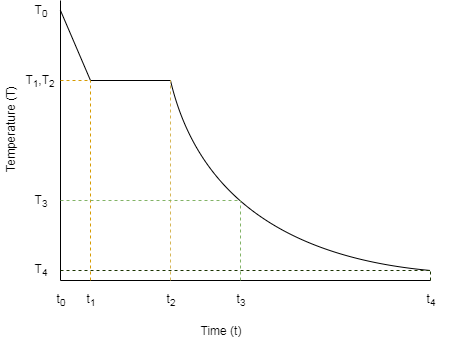
\includegraphics[width=0.75\textwidth]{regression}
	\caption{Piecewise regression breakdown of a thermocouple}
	\end{figure}

	The equation for the three piece regression is as follows: \\

	\noindent $p_1(t) =a_1t^3 + b_1t^2 + c_1t +d_1$ \\
	$p_2(t) =a_2(t-t_1)^3 + b_2(t-t_1)^2 + c_1(t-t_1) +d_2$ \\
	$p_3(t) =a_3(t-t_2)^6 + b_3(t-t_2)^5 + c_3(t-t_2)^4 +d_3(t-t_2)^3 + e_3(t-t_2)^2 +f_3(t-t_2) +g_3 $ \\

	\noindent where\\
	$d_1 = T_0$

	$p_1(t_1) = p_2(t_1)$ 
	so $d_2 = p_1(t_1) = a_1{t_1}^3 + b_1{t_1}^2 + c_1t_1 +d_1$ 

	$p_2(t_2) = p_3(t_2)$
	 so $f_3?/g_3? = p_2(t_2)= a_2(t_2-t_1)^3 + b_2(t_2-t_1)^2 + c_1(t_2-t_1) +d_2 $

\subsection*{Initial Piecewise Regression Equation Guesses} \label{Sec_PiecewiseInitial}

	\subsubsection*{Guess between $t_0$ to $t_1$}
		$p_1(t) = c_1t + d_1$ where $p_1(t_0) = T_0$ \\
		substituting $d_1 = T_0$, $p_1(t) = c_1t + T_0$ \\\\

		$p_1(t_1) = T_1$ so  $c_1t_1 + T_0 =T_1$\\
		$c_1 =\dfrac {T_1 - T_0}{t_1}$ \\

		$\therefore p_1(t) = \dfrac {T_1 - T_0}{t_1}t + T_0 $
	
	\subsubsection*{Guess between $t_1$ to $t_2$}
		$p_2(t) = c_2(t-t_1) + d_2$ where $d_2 = p_1(t_1)$ \\
		$=  c_2(t-t_1) +  p_1(t_1)$\\
		
		$p_2(t_2) = T_2$ so  $c_2(t_2 - t_1) + p_1(t_1) =T_2$\\
		$c_2 =\dfrac {T_2 - p_1(t_1)}{t_2 - t_1}$ \\

		$\therefore  p_2(t) = \dfrac {T_2 - p_1(t_1)}{t_2 - t_1}(t-t_1) +  p_1(t_1)$
	
	\subsubsection*{Guess between $t_2$ to $t_4$}
		$p_3(t) = e_3(t-t_2)^2 + f_3(t-t_2) + g_3$ \\\\
		$p_3(t_2) = T_2 = p_2(t_2) = g_3$\\
		$p_3(t_3) = T_3 = e_3(t_3-t_2)^2 + f_3(t_3-t_2) + g_3$\\
		$p_3(t_4) = T_4 = e_3(t_4-t_2)^2 + f_3(t_4-t_2) + g_3$\\\\

		Solving for $e_3$, $f_3$ with the given matrix:\\

		\[\begin{bmatrix} 
		(t_3 - t_2)^2 & (t_3 - t_2) \\
		(t_4 - t_2)^2 & (t_4 - t_2) 
		\end{bmatrix}
%
		\begin{bmatrix} 
		e_3 \\
		f_3 
		\end{bmatrix}	
%
		= 
%
		\begin{bmatrix} 
		(T_3 - f_3) \\
		(T_4 - f_3) 
		\end{bmatrix}
%
		=
%
		\begin{bmatrix} 
		(T_3 - T_2) \\
		(T_4 - T_2) 
		\end{bmatrix}\]

		Using Cramer's Rule $Ax =b$:
		
		\[A= 
%
		\begin{vmatrix} 
		(t_3 - t_2)^2 & (t_3 - t_2) \\
		(t_4 - t_2)^2 & (t_4 - t_2) 
		\end{vmatrix}
%		
		= (t_3 - t_2)^2(t_4 - t_2) - (t_4 - t_2)^2 (t_3 - t_2)\\
		\]


		\[B= 
%
		\begin{vmatrix} 
		T_3 - T_2  & (t_3 - t_2) \\
		T_4 - T_2  & (t_3 - t_2) 
		\end{vmatrix}
%		
		= (T_3 - T_2)(t_4 - t_2) - (T_4 - T_2) (t_3 - t_2)\\
		\]

		\[C= 
%
		\begin{vmatrix} 
		(t_3 - t_2)^2 & (T_3 - T_2) \\
		(t_4 - t_2)^2 & (T_4 - T_2) 
		\end{vmatrix}
%		
		= (t_3 - t_2)^2(T_4 - T_2) - (t_4 - t_2)^2 (T_3 - T_2)\\
		\]

		Finding $e_3$\\
		$e_3 = \dfrac{B}{A} = \dfrac{(T_3 - T_2)(t_4 - t_2) - (T_4 - T_2) (t_3 - t_2)}{(t_3 - t_2)^2(t_4 - t_2) - (t_4 - t_2)^2 (t_3 - t_2)}$\\

		Finding $f_3$\\
		$f_3 = \dfrac{C}{A} = \dfrac{ (t_3 - t_2)^2(T_4 - T_2) - (t_4 - t_2)^2 (T_3 - T_2)}{(t_3 - t_2)^2(t_4 - t_2) - (t_4 - t_2)^2 (t_3 - t_2)}$

\end{document}